\section{Experimental results}
\label{sect:seapp_performance}

We now present a performance evaluation of \pap.  The experiments have
been conducted on both Android 9 and 10, each with Linux kernel v4.9.
However, all the measurements shown refer to Android 10 (release
android-10.0.0\textunderscore r41).  The device used to run the tests
is a Google Pixel 3 (\emph{blueline}), in which the four \emph{gold}
cores frequency was set to 2.8 GHz, while the four \emph{silver} ones
were disabled.  The change in CPU configuration has been performed to
reduce the variability of measures.  The confidence intervals provided
have an associated confidence level of 99\%.


\subsection{App installation}

The introduction of dedicated app policies implies further steps to be
executed at app installation time, as each \pap module has to be
validated, compiled, and loaded.  To evaluate the impact on
performance, we wrote dedicated tests to stress the installation
procedure with multiple application samples.

To build representative samples of a typical consumer scenario, we
first downloaded the 150 most popular free apps from Google Play
(retrieved in October 2020)~\cite{seapp_topapps}.  The apps were
subsequently divided into three buckets: \emph{basic}, \emph{ordinary}
and \emph{huge} apps, according to the weighted normalized average of
the .apk size, the number of Android activities and the number of
services.  Based on the bucket, each app was equipped with one of the
following policy configurations: (i) \emph{basic}, 1 domain and 1 type
per policy module, (ii) \emph{ordinary}, 10 domains and 25 types, and
(iii) \emph{huge}, 20 domains and 100 types.  The rationale is that
larger apps can gain considerable benefit from the use of a large
policy.  The \emph{basic} configuration mimics how third-party apps
are currently handled, but with some key improvements, as it permits
to define the subset of services the domain can use, and it permits to
enforce app isolation, not only based on MAC category, but also
through the specification of its own type.  The \emph{ordinary} and
\emph{huge} policy configurations are meant to take full advantage of
intra-app isolation and flexibility via the definition of multiple
domains.
%
\begin{figure}[t]
	\centering
	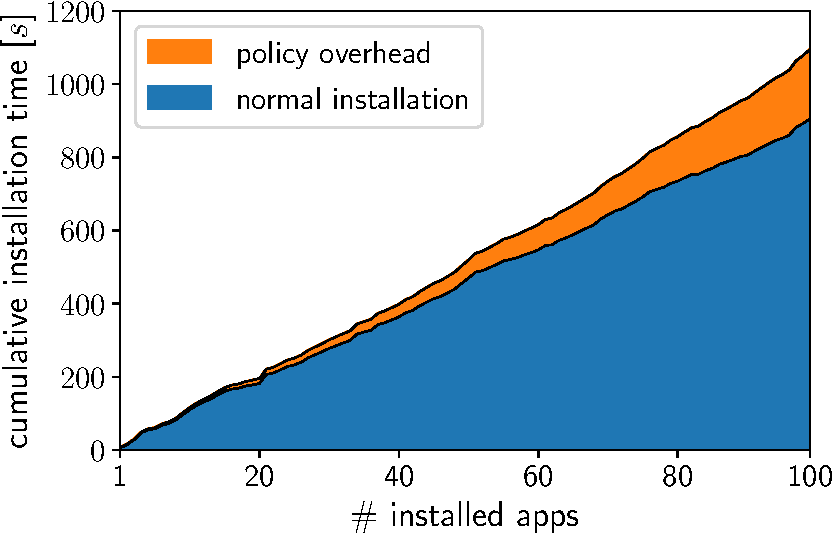
\includegraphics[width=0.7\columnwidth]{chapters/seapp/data/top100_cumulative}
	\caption{\label{fig:seapp_benchmark100} Cumulative install time
          overhead when installing the top 100 free apps on Google
          Play Store with our policies}
\end{figure}
%
Each test was repeated five times, measuring the time each package
took to install.  The measurements were done with the *nix {\em date}
utility.

\noindent{\bf Test I.}
To measure the overhead caused by the presence of the policy module,
we performed on device installation of each of the previously
described app buckets (\emph{basic}, \emph{ordinary} and \emph{huge})
via Android Debug Bridge (adb)~\cite{seapp_adblink}.

The results of Test I are illustrated in
Figure~\ref{fig:seapp_three_kinds}.  In detail, it shows in blue
(i.e., the lower part of the bar) the time required by the system to
install the current package without the dedicated policy module, while
in orange (i.e., the top of the bar) the overhead caused by the
presence of the policy module.  The data report that a limited
overhead is associated with apps with \textit{huge} policies, at most
$3.59 \pm 0.04 s$, while \textit{basic} and \textit{ordinary} policy
configurations exhibit a negligible slowdown, never exceeding
$1.22 \pm 0.02 s$.

\noindent{\bf Test II.}
To evaluate the overall impact of \pap in a typical consumer scenario,
we performed a test evaluating cumulative installations.  At first, we
repeated the installation of the top 100 apps on Google Play Store
with the same policy configuration as in Test I (see
Figure~\ref{fig:seapp_benchmark100}).  In this case, we measured an
overhead of $20.98 \pm 1,31\%$ on total installation time.

As explained in Section~\ref{sect:seapp_implementation}, each time a
new application is installed, all policy fragments stored in the
device have to be recompiled to produce the new binary policy.  The
installation time overhead then grows with the increase in the number
of installed policy modules.  To further analyze this aspect, we
repeated the installation of the top 100 free apps adding to all the
packages in three separate experiments the same \textit{basic},
\textit{ordinary}, and \textit{huge} policy configurations.  The
experimental results illustrated in
Figure~\ref{fig:seapp_install_time}, show that only the use of {\em
  huge} policy modules introduces a non-negligible overhead
($45.35 \pm 2.44\%$ on total installation time).  However, this policy
configuration simulates an edge case, as we do not expect to find 100
of them in a real scenario. To give a comparison, the {\em huge}
policy declares 100 types; {\tt public/file.te}, i.e., the file used
to define all the file types of the system, declares 314 types in
Android 10.

In Table~\ref{tab:seapp_policy} we report the sizes of the overall
policies for the three scenarios considered in this experiment.  We
report the number of MAC types, the number of produced AV rules, and
the overall size in KBytes of the binary policy.
%
\begin{table}[h!]
	\centering
        \small
	\begin{tabular}{|l|r|r|r|}
		\hline
		\textbf{policy} & \textbf{\#types} & \textbf{\#avrules} & \textbf{KB} \\ \hline
		system & 1536 & 29228 &  596 \\ \hline
		system + 100 basic & 1836 & 47028 &  867 \\ \hline
		system + 100 ordinary & 6036 & 213228 &  3512 \\ \hline
		system + 100 huge & 15536 & 417228 &  7064 \\ \hline
	\end{tabular}
	\caption{Policy size}
	\label{tab:seapp_policy}
\end{table}
%
\begin{figure}[t]
	\centering
	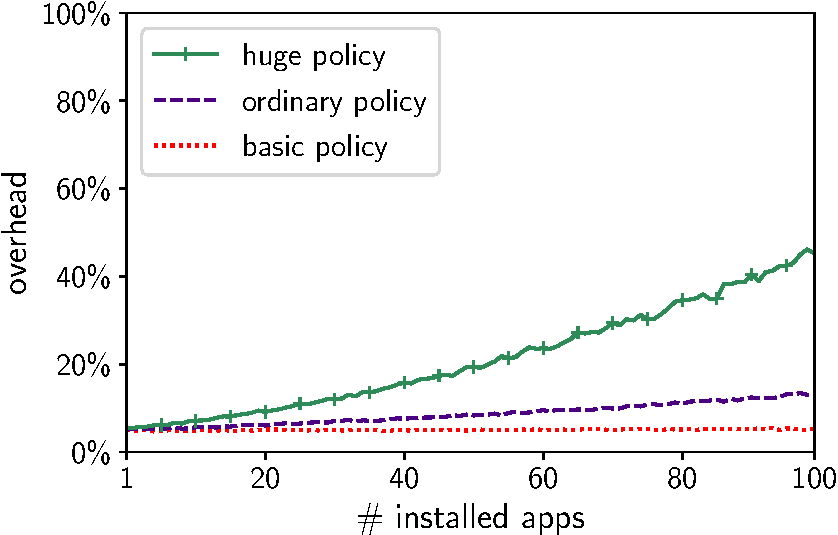
\includegraphics[width=0.7\columnwidth]{chapters/seapp/data/overheads}
	\caption{\label{fig:seapp_install_time} Install time overhead for the three policy sizes}
\end{figure}


\subsection{Runtime performance}

We now evaluate the runtime overhead for an app taking full advantage
of \pap.  We focus on the creation of processes and files, as they are
the entities directly affected by the changes made in the
implementation.  The data shown refer to the creation time of each
resource.  The measurements have been acquired via
\textit{System.nanoTime} and have been repeated 100 times for each
test.  Also, all outliers diverging more than 3 standard deviations
from the mean have been suppressed.


\subsubsection{Processes}

As discussed in Section~\ref{sect:seapp_implementation}, in \pap the
creation of a process is originated from the request of execution of
an Android component.  Thus, the slowdown occurs between the request
for the component and the execution of the method \textit{onCreate},
which is the time interval subject to measurement.  Our evaluation is
limited to activities and services, as these are the components most
used by developers.  Our analysis showed identical behavior for
broadcast receivers and content providers, the other two components
supporting the \process attribute in the manifest.

Separate test cases have been identified based on the type of process
that supports the component.  We refer to \emph{Local}, \emph{Remote},
\emph{Isolated} or \emph{\pap} components when we run components
respectively in the current process, in another process, in another
process with the \isolatedapp domain (using the {\em isolatedprocess}
we described in Section~\ref{sect:seapp_int_comp_isolation}), or in a
package specific domain (declared in the app policy module).
Furthermore, we cover \emph{cold} and \emph{warm} start scenarios.
The {\em cold} start corresponds to the first time the application
brings up the component, and the {\em warm} start to the subsequent
times the app reuses a previously instantiated one.

\begin{table}[h]
  \centering
  \small
  \begin{tabular}{|l|c|c|c|c|c|c|c|c|} \cline{2-9}
    \multicolumn{1}{c|}{}&\multicolumn{4}{c|}{\textbf{Cold start
                           (ms)}}&\multicolumn{4}{c|}{\textbf{Warm start (ms)}} \\
    \cline{1-9}

    \multicolumn{1}{|c|}{\multirow{2}{*}{\textbf{\emph{Component}}}}&\multicolumn{2}{c|}{\textbf{\emph{Stock OS}}}&\multicolumn{2}{c|}{\textbf{\emph{\pap}}}&\multicolumn{2}{c|}{\textbf{\emph{Stock OS}}}&\multicolumn{2}{c|}{\textbf{\emph{\pap}}}  \\ \cline{2-9}

    \multicolumn{1}{|c|}{}  & $\mu$ & $\sigma$ & $\mu$ & $\sigma$ & $\mu$ & $\sigma$ & $\mu$ & $\sigma$   \\ \hline

        LocalActivity		& 39.102	& 1.094	& 38.689	& 0.980	& 21.052	& 6.046	& 18.685	& 5.001	\\ \cline{1-9}
        RemoteActivity	& 123.468	& 3.176	& 124.649	& 3.526	& 15.722	& 2.682	& 15.933	& 3.256	\\ \cline{1-9}
        \pap Activity		& -			& -		& 127.356	& 3.542	& -			& -		& 15.188	& 2.394	\\ \cline{1-9}

    \hline \hline

        LocalService		& 19.164	& 1.444	& 18.835	& 1.392	& 1.399	& 0.208	& 1.328	& 0.208	\\ \cline{1-9}
        RemoteService		& 105.467	& 2.800	& 106.935	& 2.565	& 2.617	& 0.879	& 2.676	& 0.593	\\ \cline{1-9}
        IsolatedService	& 103.923	& 2.425	& 104.260	& 3.727	& -		& -		& -		& -		\\ \cline{1-9}
        \pap Service		& -			& -		& 106.925	& 3.774	& -		& -		& 2.528	& 0.675 \\ \cline{1-9}
  \end{tabular}
  \caption{Cold and warm start performance for activities and
    services}
  \label{tab:seapp_start_2}
\end{table}

The results shown in Table~\ref{tab:seapp_start_2} demonstrate that
the performance of a stock version of the OS and \pap are equivalent.
Also, we observe that apps willing to benefit of the intra-app
isolation feature get from the use of \pap the same performance they
would get from the use of remote components.  Our approach also proves
to outperform the \textit{IsolatedService}, as the {\em
  isolatedprocess} option forces the creation of a new process every
time an {\em IsolatedService} that was previously {\em unBind}-ed is
activated.  This introduces a slowdown of $102 \pm 1 ms$ compared to
the {\em SEAppService} warm start, which instead benefits from the
system caching mechanism.

\subsubsection{Files}

Alongside the usual creation method, \pap introduces in Android the
possibility of creating files with a security domain defined by the
app dedicated \filecontexts.  Table~\ref{tab:seapp_file_creation}
shows the time required to create a file, for each of the methods
discussed.  We observe no overhead on direct file creation, but the
overall execution time becomes larger due to the invocation, as
described in Section \ref{sect:seapp_app_runtime}, of the \restorecon
service, which requires approximately $374 \pm 30\mu s$.  This
overhead only occurs at file creation and every subsequent operation
on the file does not exhibit any performance degradation.

\begin{table}[h]
  \small \centering
  \begin{tabular}{|l|c|c|}
    \hline
    \multicolumn{3}{|c|}{\textbf{File creation}}  \\ \hline \hline
    \textbf{\textit{Test}} & \textbf{$\mu$ (\textmu s)} & \textbf{$\sigma$ (\textmu s)} \\ \hline
        Stock OS			&  57.077	&  5.174		\\ \hline
        \pap				&  60.696	&  6.782		\\ \hline
        \pap +                          & \multirow{2}{*}{431.472} & \multirow{2}{*}{109.494} \\
        \restorecon & & \\ \hline
  \end{tabular}
  \caption{File creation performance}
  \label{tab:seapp_file_creation}
\end{table}


%%% Local Variables: 
%%% mode: latex
%%% TeX-master: "../../../main.tex"
%%% reftex-default-bibliography: "../../../bib/biblio.bib"
%%% End: